%preamble
\documentclass{beamer} % use the beamer package for presentations
% \documentclass[notes=only]{beamer} %compile with this line uncommented to produce speaker notes
\usetheme{metropolis} % use the metropolis theme
\usepackage{wrapfig} % for text wrapping around figures

% used for formatting code blocks
\usepackage[most]{tcolorbox}

% sets the location of the graphics directory
\graphicspath{ {./assets/images/} }

% title slide setup
\title{Methods in \\Research Software Engineering}
\date{6th May 2021}
\author{Dr David Wilby}
\institute{Research Software Engineering Team,\\ The University of Sheffield}
\titlegraphic{\vspace*{4cm}\hspace*{7cm}
\includegraphics[width=.3\textwidth]{RSE_logo_blackborder}}

% the main document
\begin{document}

  \begin{frame}
    \titlepage
  \end{frame}

  \begin{frame}{Outline}
    \begin{itemize}
      \item Introduction
      \item Academic Research
      \item Research Software Engineering
      \item Version Control
      \item GitHub (collaboration \& project management)
      \item Best Practice
      \begin{itemize}
        \item Documentation
        \item Commenting
        \item Code Style
        \item Testing
        \item Licenses
        \item Repository Organisation
      \end{itemize}
      \item Resources
      \item Nuggets of Wisdom
    \end{itemize}
  \end{frame}

  \begin{frame}{About Me}

    \begin{wrapfigure}{r}{0.3\textwidth}
        
\includegraphics[width=0.3\textwidth]{wilby}
    \end{wrapfigure}

    David Wilby

    \href{https://davidwilby.github.io/}{davidwilby.github.io/}

    \textbf{Who?}
    
    Research Software Engineer

    \textbf{Background}

    Optical Physics, Sensory Biology, Numerical Simulation, HPC

    \textbf{Interests}

    Python, Git, Matlab, Open Source, Web Apps, Research Impact

  \end{frame}

  \begin{frame}{Academic Research}
    \begin{center}
      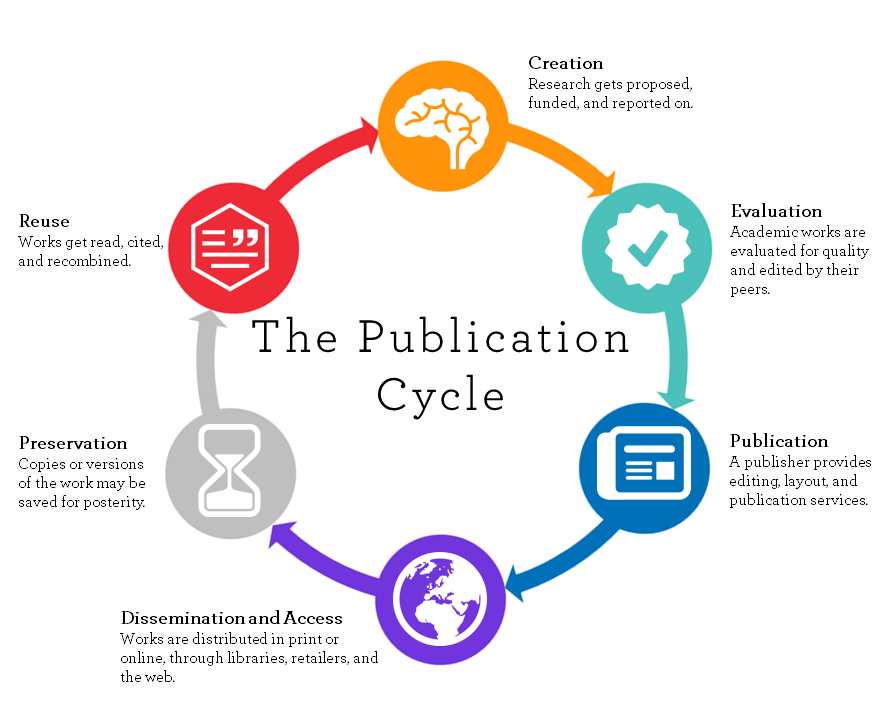
\includegraphics[height=.8\textheight]{publication_cycle.png}
    \end{center}
    \tiny{Image: \href{https://press.rebus.community/literaturereviewsedunursing/chapter/chapter-2-what-is-a-literature-review/}{Rebus community}}
  \end{frame}

  \begin{frame}{Research Software Engineering}
    \begin{columns}
      \begin{column}{0.4\textwidth}
        \textbf{Goals}
        \begin{itemize}
          \item reproducibility
          \item transparency
          \item accountability
          \item exendability
          \item lifespan
          \item impact
        \end{itemize}
        
        \textbf{Methods}
        \begin{itemize}
          \item version control
          \item open source code
          \item reliable code
          \item documentation
        \end{itemize}
      \end{column}

      \begin{column}{0.6\textwidth}
        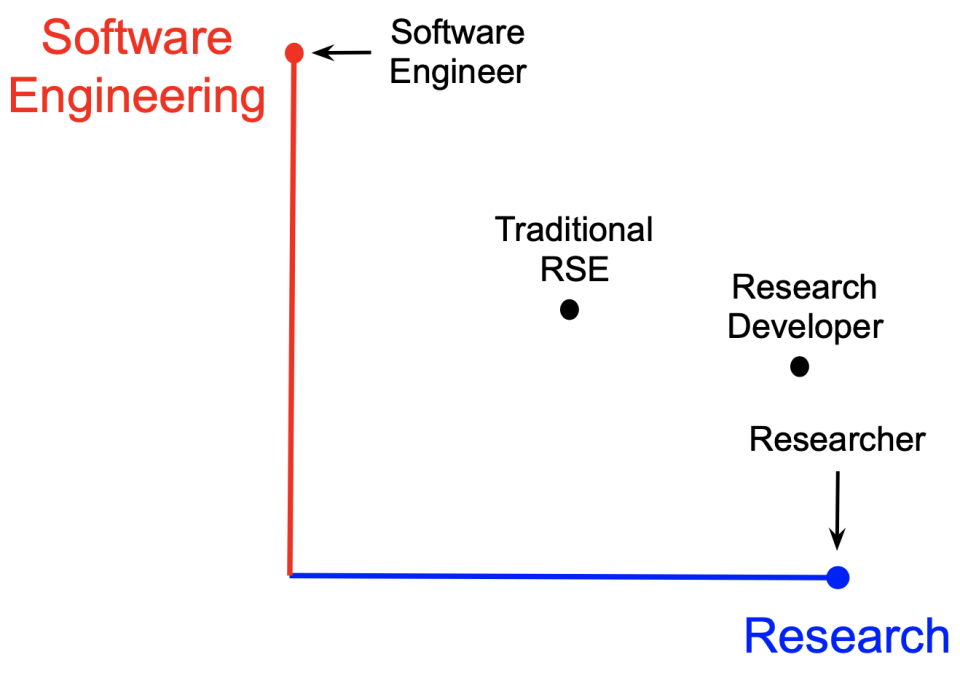
\includegraphics[width=\textwidth]{RSE_graph_katz.png}
        \tiny{Image: \href{https://danielskatzblog.wordpress.com/2019/07/12/super-rses-combining-research-and-service-in-three-dimensions-of-research-software-engineering/}{\underline{Daniel S. Katz}}}
      \end{column}
  \end{columns}
  \end{frame}


% Version Control
  \begin{frame}{Why use version control?}

    \begin{itemize}
      \item try new ideas,
      \item confidence,
      \item ease of backing up (on remotes),
      \item collaboration,
    \end{itemize}
    
  \end{frame}


  \begin{frame}{Version Control}
    Ways to use Git:
    \begin{itemize}
      \item \href{https://git-scm.com/}{Command Line Git 
\includegraphics[height=.05\textheight]{git}}
      \item \href{https://code.visualstudio.com/}{VS Code 
\includegraphics[height=.05\textheight]{vscode}}
      \item \href{https://www.gitkraken.com/}{GitKraken 
\includegraphics[height=.05\textheight]{gitkraken}}
      \item \href{https://gitforwindows.org/}{Git Bash 
\includegraphics[height=.07\textheight]{gitbash}}
      \item + many more...
    \end{itemize}

  \end{frame}



  \begin{frame}{Git learning resources}

  \begin{itemize}
    \item \href{http://swcarpentry.github.io/git-novice/}{\underline{software carpentry lesson}}
    \item \textit{"oh sh** git"} - \href{https://wizardzines.com/zines/oh-shit-git/}{\underline{zine}}, or \href{https://ohshitgit.com/}{\underline{blog}}
    \item \href{https://the-turing-way.netlify.app/reproducible-research/vcs.html}{\underline{The Turing Way}}
    \item \href{https://stackoverflow.com/}{\underline{stack overflow}} \textit{etc.} - \textit{use carefully}
    \item blogs on \href{https://dev.to/}{\underline{dev}} or \href{https://www.atlassian.com/git/tutorials}{\underline{atlassian}} \textit{etc.}
  \end{itemize}

  \end{frame}



  \begin{frame}[fragile]{Git - useful commands}
    \begin{tcblisting}{beamer,colback=black,colupper=white,colframe=black,
      listing only,listing options={style=tcblatex,language=sh},hbox,
      every listing line*={\textcolor{cyan}{\small\ttfamily\bfseries\$}}}
  git status
    \end{tcblisting}
    Show current branch, staged/tracked/untracked files, current status.
    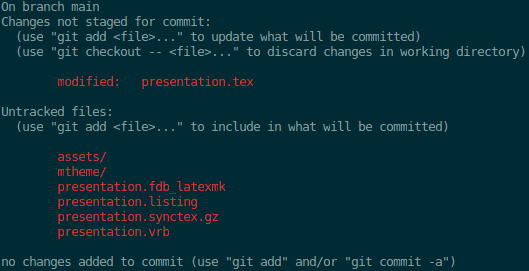
\includegraphics[height=.6\textheight]{git_status_output.png}
  \end{frame}

  \begin{frame}[fragile]
    'stash' your current unstaged changes.\newline
    \begin{tcblisting}{beamer,colback=black,colupper=white,colframe=black,
      listing only,listing options={style=tcblatex,language=sh},hbox,
      every listing line*={\textcolor{cyan}{\small\ttfamily\bfseries\$}}}
  git stash
    \end{tcblisting}
    
    \begin{tcblisting}{beamer,colback=black,colupper=white,colframe=black,
      listing only,listing options={style=tcblatex,language=sh},hbox}
> Saved working directory and index state WIP on main: 3a158fc add some notes
    \end{tcblisting}

    Another couple to try:
    \begin{tcblisting}{beamer,colback=black,colupper=white,colframe=black,
      listing only,listing options={style=tcblatex,language=sh},hbox,
      every listing line*={\textcolor{cyan}{\small\ttfamily\bfseries\$}}}
  git stash list
    \end{tcblisting}

    \begin{tcblisting}{beamer,colback=black,colupper=white,colframe=black,
      listing only,listing options={style=tcblatex,language=sh},hbox,
      every listing line*={\textcolor{cyan}{\small\ttfamily\bfseries\$}}}
  git stash pop
    \end{tcblisting}
    
  \end{frame}

  \begin{frame}[fragile]
    
    \begin{tcblisting}{beamer,colback=black,colupper=white,colframe=black,
      listing only,listing options={style=tcblatex,language=sh},hbox,
      every listing line*={\textcolor{cyan}{\small\ttfamily\bfseries\$}}}
  git remote -v
    \end{tcblisting}
    
    \begin{tcblisting}{beamer,colback=black,colupper=white,colframe=black,
      listing only,listing options={style=tcblatex,language=sh},hbox}
> origin git@github.com:davidwilby/ResearchSoftwareMethods (fetch)
> origin git@github.com:davidwilby/ResearchSoftwareMethods (push)
    \end{tcblisting}

  \end{frame}

  \begin{frame}[fragile]
    \begin{tcblisting}{beamer,colback=black,colupper=white,colframe=black,
      listing only,listing options={style=tcblatex,language=sh},hbox,
      every listing line*={\textcolor{cyan}{\small\ttfamily\bfseries\$}}}
  git log --decorate --all --oneline --graph
    \end{tcblisting}
    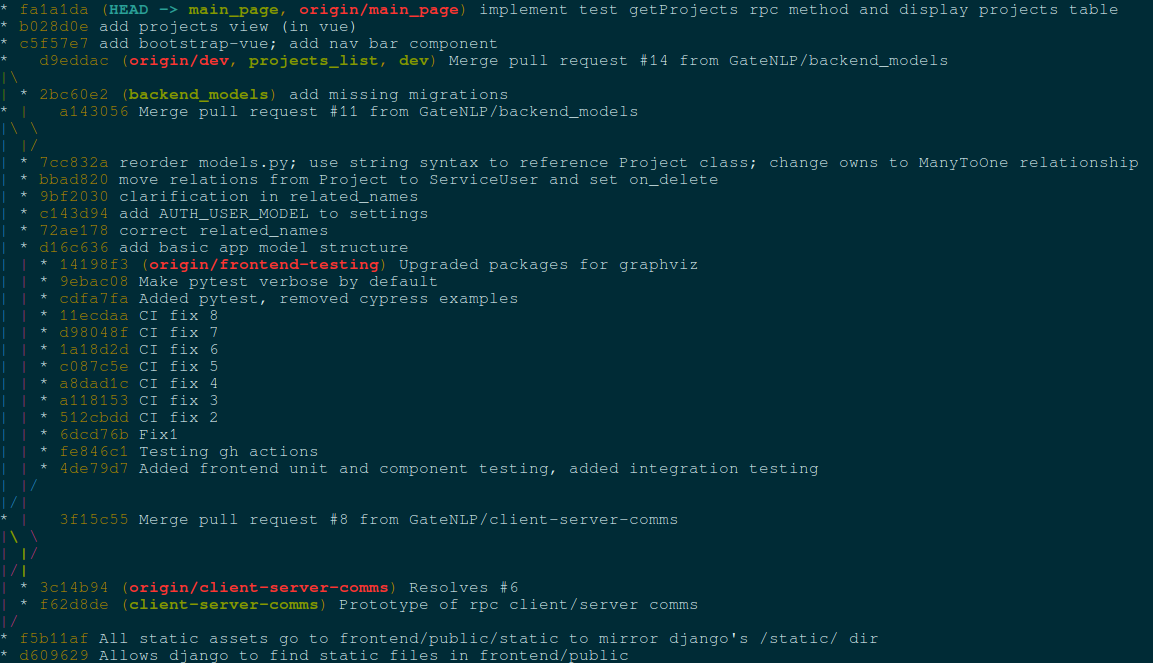
\includegraphics[height=.9\textheight]{git_log_tree_output.png}
  \end{frame}


  \begin{frame}{GitHub - collaboration}
    \begin{itemize}
      \item 
    \end{itemize}
  \end{frame}

  \begin{frame}{GitHub - project management}
  \end{frame}

  \begin{frame}{Best practice - documentation}
  \end{frame}

  \begin{frame}{Best practice - testing}
  \end{frame}

  \begin{frame}{Best practice - code style}
    \pause
    \begin{itemize}
      \item Comments
      \item Conciseness
      \item DRY - Don't Repeat Yourself
      \item Modularity
    \end{itemize}
  \end{frame}

  \begin{frame}[fragile]{Best practice - project organisation}
    \begin{columns}
      \begin{column}{0.3\textwidth}
        \small
        \begin{verbatim}
data/
docs/
figs/
output/
src/
tests/
01_ingest_data.R
02_clean_data.R
03_exploratory_analysis.R
04_fit_models.R
05_generate_figures.R
analysis_example.Rproj
README.md\end{verbatim}
      \end{column}  
      \begin{column}{0.5\textwidth}
        \begin{itemize}
          \item be consistent
          \item include a license
          \item machine readable filenames
        \end{itemize}
      \end{column}  
  \end{columns}
  \end{frame}

  \note[itemize]{
  \item human readable filenames
  \item file specific READme files
  }

  \begin{frame}{Best practice - environment management}
  \end{frame}

  \begin{frame}{HPC Resources at Sheffield}
    Why use HPC?
    \begin{itemize}
      \item Parallel computing
      \item Batch management
      \item Access to GPUs
      \item Run analysis elsewhere
      \item Efficiency
    \end{itemize}

    Resources available:
    Tier 3 (university-specific):
    \begin{itemize}
      \item ShARC
      \item Bessemer
    \end{itemize}

  \end{frame}

  \begin{frame}{Key Points}
    \begin{itemize}
      \item document, document, document
      \item keep things simple
      \item isolate environments
      \item version code \& data
      \item try your best!
    \end{itemize}
  \end{frame}

  \begin{frame}{Resources}
    \begin{itemize}
      \item \href{https://www.britishecologicalsociety.org/wp-content/uploads/2017/12/guide-to-reproducible-code.pdf}{\underline{BES Guide to Reproducible Research Code}}
      \item \href{https://the-turing-way.netlify.app/}{\underline{The Turing Way}}
    \end{itemize}
  \end{frame}

\end{document}
